
%% bare_conf.tex
%% V1.3
%% 2007/01/11
%% by Michael Shell
%% See:
%% http://www.michaelshell.org/
%% for current contact information.
%%
%% This is a skeleton file demonstrating the use of IEEEtran.cls
%% (requires IEEEtran.cls version 1.7 or later) with an IEEE conference paper.
%%
%% Support sites:
%% http://www.michaelshell.org/tex/ieeetran/
%% http://www.ctan.org/tex-archive/macros/latex/contrib/IEEEtran/
%% and
%% http://www.ieee.org/

%%*************************************************************************
%% Legal Notice:
%% This code is offered as-is without any warranty either expressed or
%% implied; without even the implied warranty of MERCHANTABILITY or
%% FITNESS FOR A PARTICULAR PURPOSE! 
%% User assumes all risk.
%% In no event shall IEEE or any contributor to this code be liable for
%% any damages or losses, including, but not limited to, incidental,
%% consequential, or any other damages, resulting from the use or misuse
%% of any information contained here.
%%
%% All comments are the opinions of their respective authors and are not
%% necessarily endorsed by the IEEE.
%%
%% This work is distributed under the LaTeX Project Public License (LPPL)
%% ( http://www.latex-project.org/ ) version 1.3, and may be freely used,
%% distributed and modified. A copy of the LPPL, version 1.3, is included
%% in the base LaTeX documentation of all distributions of LaTeX released
%% 2003/12/01 or later.
%% Retain all contribution notices and credits.
%% ** Modified files should be clearly indicated as such, including  **
%% ** renaming them and changing author support contact information. **
%%
%% File list of work: IEEEtran.cls, IEEEtran_HOWTO.pdf, bare_adv.tex,
%%                    bare_conf.tex, bare_jrnl.tex, bare_jrnl_compsoc.tex
%%*************************************************************************

% *** Authors should verify (and, if needed, correct) their LaTeX system  ***
% *** with the testflow diagnostic prior to trusting their LaTeX platform ***
% *** with production work. IEEE's font choices can trigger bugs that do  ***
% *** not appear when using other class files.                            ***
% The testflow support page is at:
% http://www.michaelshell.org/tex/testflow/



% Note that the a4paper option is mainly intended so that authors in
% countries using A4 can easily print to A4 and see how their papers will
% look in print - the typesetting of the document will not typically be
% affected with changes in paper size (but the bottom and side margins will).
% Use the testflow package mentioned above to verify correct handling of
% both paper sizes by the user's LaTeX system.
%
% Also note that the "draftcls" or "draftclsnofoot", not "draft", option
% should be used if it is desired that the figures are to be displayed in
% draft mode.
%
\documentclass[conference]{IEEEtran}
\usepackage{blindtext, graphicx}
% Add the compsoc option for Computer Society conferences.
%
% If IEEEtran.cls has not been installed into the LaTeX system files,
% manually specify the path to it like:
% \documentclass[conference]{../sty/IEEEtran}





% Some very useful LaTeX packages include:
% (uncomment the ones you want to load)


% *** MISC UTILITY PACKAGES ***
%
%\usepackage{ifpdf}
% Heiko Oberdiek's ifpdf.sty is very useful if you need conditional
% compilation based on whether the output is pdf or dvi.
% usage:
% \ifpdf
%   % pdf code
% \else
%   % dvi code
% \fi
% The latest version of ifpdf.sty can be obtained from:
% http://www.ctan.org/tex-archive/macros/latex/contrib/oberdiek/
% Also, note that IEEEtran.cls V1.7 and later provides a builtin
% \ifCLASSINFOpdf conditional that works the same way.
% When switching from latex to pdflatex and vice-versa, the compiler may
% have to be run twice to clear warning/error messages.






% *** CITATION PACKAGES ***
%
%\usepackage{cite}
% cite.sty was written by Donald Arseneau
% V1.6 and later of IEEEtran pre-defines the format of the cite.sty package
% \cite{} output to follow that of IEEE. Loading the cite package will
% result in citation numbers being automatically sorted and properly
% "compressed/ranged". e.g., [1], [9], [2], [7], [5], [6] without using
% cite.sty will become [1], [2], [5]--[7], [9] using cite.sty. cite.sty's
% \cite will automatically add leading space, if needed. Use cite.sty's
% noadjust option (cite.sty V3.8 and later) if you want to turn this off.
% cite.sty is already installed on most LaTeX systems. Be sure and use
% version 4.0 (2003-05-27) and later if using hyperref.sty. cite.sty does
% not currently provide for hyperlinked citations.
% The latest version can be obtained at:
% http://www.ctan.org/tex-archive/macros/latex/contrib/cite/
% The documentation is contained in the cite.sty file itself.






% *** GRAPHICS RELATED PACKAGES ***
%
\ifCLASSINFOpdf
  % \usepackage[pdftex]{graphicx}
  % declare the path(s) where your graphic files are
  % \graphicspath{{../pdf/}{../jpeg/}}
  % and their extensions so you won't have to specify these with
  % every instance of \includegraphics
  % \DeclareGraphicsExtensions{.pdf,.jpeg,.png}
\else
  % or other class option (dvipsone, dvipdf, if not using dvips). graphicx
  % will default to the driver specified in the system graphics.cfg if no
  % driver is specified.
  % \usepackage[dvips]{graphicx}
  % declare the path(s) where your graphic files are
  % \graphicspath{{../eps/}}
  % and their extensions so you won't have to specify these with
  % every instance of \includegraphics
  % \DeclareGraphicsExtensions{.eps}
\fi
% graphicx was written by David Carlisle and Sebastian Rahtz. It is
% required if you want graphics, photos, etc. graphicx.sty is already
% installed on most LaTeX systems. The latest version and documentation can
% be obtained at: 
% http://www.ctan.org/tex-archive/macros/latex/required/graphics/
% Another good source of documentation is "Using Imported Graphics in
% LaTeX2e" by Keith Reckdahl which can be found as epslatex.ps or
% epslatex.pdf at: http://www.ctan.org/tex-archive/info/
%
% latex, and pdflatex in dvi mode, support graphics in encapsulated
% postscript (.eps) format. pdflatex in pdf mode supports graphics
% in .pdf, .jpeg, .png and .mps (metapost) formats. Users should ensure
% that all non-photo figures use a vector format (.eps, .pdf, .mps) and
% not a bitmapped formats (.jpeg, .png). IEEE frowns on bitmapped formats
% which can result in "jaggedy"/blurry rendering of lines and letters as
% well as large increases in file sizes.
%
% You can find documentation about the pdfTeX application at:
% http://www.tug.org/applications/pdftex





% *** MATH PACKAGES ***
%
%\usepackage[cmex10]{amsmath}
% A popular package from the American Mathematical Society that provides
% many useful and powerful commands for dealing with mathematics. If using
% it, be sure to load this package with the cmex10 option to ensure that
% only type 1 fonts will utilized at all point sizes. Without this option,
% it is possible that some math symbols, particularly those within
% footnotes, will be rendered in bitmap form which will result in a
% document that can not be IEEE Xplore compliant!
%
% Also, note that the amsmath package sets \interdisplaylinepenalty to 10000
% thus preventing page breaks from occurring within multiline equations. Use:
%\interdisplaylinepenalty=2500
% after loading amsmath to restore such page breaks as IEEEtran.cls normally
% does. amsmath.sty is already installed on most LaTeX systems. The latest
% version and documentation can be obtained at:
% http://www.ctan.org/tex-archive/macros/latex/required/amslatex/math/





% *** SPECIALIZED LIST PACKAGES ***
%
%\usepackage{algorithmic}
% algorithmic.sty was written by Peter Williams and Rogerio Brito.
% This package provides an algorithmic environment fo describing algorithms.
% You can use the algorithmic environment in-text or within a figure
% environment to provide for a floating algorithm. Do NOT use the algorithm
% floating environment provided by algorithm.sty (by the same authors) or
% algorithm2e.sty (by Christophe Fiorio) as IEEE does not use dedicated
% algorithm float types and packages that provide these will not provide
% correct IEEE style captions. The latest version and documentation of
% algorithmic.sty can be obtained at:
% http://www.ctan.org/tex-archive/macros/latex/contrib/algorithms/
% There is also a support site at:
% http://algorithms.berlios.de/index.html
% Also of interest may be the (relatively newer and more customizable)
% algorithmicx.sty package by Szasz Janos:
% http://www.ctan.org/tex-archive/macros/latex/contrib/algorithmicx/




% *** ALIGNMENT PACKAGES ***
%
%\usepackage{array}
% Frank Mittelbach's and David Carlisle's array.sty patches and improves
% the standard LaTeX2e array and tabular environments to provide better
% appearance and additional user controls. As the default LaTeX2e table
% generation code is lacking to the point of almost being broken with
% respect to the quality of the end results, all users are strongly
% advised to use an enhanced (at the very least that provided by array.sty)
% set of table tools. array.sty is already installed on most systems. The
% latest version and documentation can be obtained at:
% http://www.ctan.org/tex-archive/macros/latex/required/tools/


%\usepackage{mdwmath}
%\usepackage{mdwtab}
% Also highly recommended is Mark Wooding's extremely powerful MDW tools,
% especially mdwmath.sty and mdwtab.sty which are used to format equations
% and tables, respectively. The MDWtools set is already installed on most
% LaTeX systems. The lastest version and documentation is available at:
% http://www.ctan.org/tex-archive/macros/latex/contrib/mdwtools/


% IEEEtran contains the IEEEeqnarray family of commands that can be used to
% generate multiline equations as well as matrices, tables, etc., of high
% quality.


%\usepackage{eqparbox}
% Also of notable interest is Scott Pakin's eqparbox package for creating
% (automatically sized) equal width boxes - aka "natural width parboxes".
% Available at:
% http://www.ctan.org/tex-archive/macros/latex/contrib/eqparbox/





% *** SUBFIGURE PACKAGES ***
%\usepackage[tight,footnotesize]{subfigure}
% subfigure.sty was written by Steven Douglas Cochran. This package makes it
% easy to put subfigures in your figures. e.g., "Figure 1a and 1b". For IEEE
% work, it is a good idea to load it with the tight package option to reduce
% the amount of white space around the subfigures. subfigure.sty is already
% installed on most LaTeX systems. The latest version and documentation can
% be obtained at:
% http://www.ctan.org/tex-archive/obsolete/macros/latex/contrib/subfigure/
% subfigure.sty has been superceeded by subfig.sty.



%\usepackage[caption=false]{caption}
%\usepackage[font=footnotesize]{subfig}
% subfig.sty, also written by Steven Douglas Cochran, is the modern
% replacement for subfigure.sty. However, subfig.sty requires and
% automatically loads Axel Sommerfeldt's caption.sty which will override
% IEEEtran.cls handling of captions and this will result in nonIEEE style
% figure/table captions. To prevent this problem, be sure and preload
% caption.sty with its "caption=false" package option. This is will preserve
% IEEEtran.cls handing of captions. Version 1.3 (2005/06/28) and later 
% (recommended due to many improvements over 1.2) of subfig.sty supports
% the caption=false option directly:
%\usepackage[caption=false,font=footnotesize]{subfig}
%
% The latest version and documentation can be obtained at:
% http://www.ctan.org/tex-archive/macros/latex/contrib/subfig/
% The latest version and documentation of caption.sty can be obtained at:
% http://www.ctan.org/tex-archive/macros/latex/contrib/caption/




% *** FLOAT PACKAGES ***
%
%\usepackage{fixltx2e}
% fixltx2e, the successor to the earlier fix2col.sty, was written by
% Frank Mittelbach and David Carlisle. This package corrects a few problems
% in the LaTeX2e kernel, the most notable of which is that in current
% LaTeX2e releases, the ordering of single and double column floats is not
% guaranteed to be preserved. Thus, an unpatched LaTeX2e can allow a
% single column figure to be placed prior to an earlier double column
% figure. The latest version and documentation can be found at:
% http://www.ctan.org/tex-archive/macros/latex/base/



%\usepackage{stfloats}
% stfloats.sty was written by Sigitas Tolusis. This package gives LaTeX2e
% the ability to do double column floats at the bottom of the page as well
% as the top. (e.g., "\begin{figure*}[!b]" is not normally possible in
% LaTeX2e). It also provides a command:
%\fnbelowfloat
% to enable the placement of footnotes below bottom floats (the standard
% LaTeX2e kernel puts them above bottom floats). This is an invasive package
% which rewrites many portions of the LaTeX2e float routines. It may not work
% with other packages that modify the LaTeX2e float routines. The latest
% version and documentation can be obtained at:
% http://www.ctan.org/tex-archive/macros/latex/contrib/sttools/
% Documentation is contained in the stfloats.sty comments as well as in the
% presfull.pdf file. Do not use the stfloats baselinefloat ability as IEEE
% does not allow \baselineskip to stretch. Authors submitting work to the
% IEEE should note that IEEE rarely uses double column equations and
% that authors should try to avoid such use. Do not be tempted to use the
% cuted.sty or midfloat.sty packages (also by Sigitas Tolusis) as IEEE does
% not format its papers in such ways.





% *** PDF, URL AND HYPERLINK PACKAGES ***
%
%\usepackage{url}
% url.sty was written by Donald Arseneau. It provides better support for
% handling and breaking URLs. url.sty is already installed on most LaTeX
% systems. The latest version can be obtained at:
% http://www.ctan.org/tex-archive/macros/latex/contrib/misc/
% Read the url.sty source comments for usage information. Basically,
% \url{my_url_here}.





% *** Do not adjust lengths that control margins, column widths, etc. ***
% *** Do not use packages that alter fonts (such as pslatex).         ***
% There should be no need to do such things with IEEEtran.cls V1.6 and later.
% (Unless specifically asked to do so by the journal or conference you plan
% to submit to, of course. )


% correct bad hyphenation here
\hyphenation{op-tical net-works semi-conduc-tor}


\begin{document}
%
% paper title
% can use linebreaks \\ within to get better formatting as desired
\title{Schema Matching using Machine Learning}


% author names and affiliations
% use a multiple column layout for up to three different
% affiliations


\author{\IEEEauthorblockN{Ankita Mehta}
\and
\IEEEauthorblockN{Shruti Jadon}
\and
\IEEEauthorblockN{Tanvi Sahay}
}

% conference papers do not typically use \thanks and this command
% is locked out in conference mode. If really needed, such as for
% the acknowledgment of grants, issue a \IEEEoverridecommandlockouts
% after \documentclass

% for over three affiliations, or if they all won't fit within the width
% of the page, use this alternative format:
% 
%\author{\IEEEauthorblockN{Michael Shell\IEEEauthorrefmark{1},
%Homer Simpson\IEEEauthorrefmark{2},
%James Kirk\IEEEauthorrefmark{3}, 
%Montgomery Scott\IEEEauthorrefmark{3} and
%Eldon Tyrell\IEEEauthorrefmark{4}}
%\IEEEauthorblockA{\IEEEauthorrefmark{1}School of Electrical and Computer Engineering\\
%Georgia Institute of Technology,
%Atlanta, Georgia 30332--0250\\ Email: see http://www.michaelshell.org/contact.html}
%\IEEEauthorblockA{\IEEEauthorrefmark{2}Twentieth Century Fox, Springfield, USA\\
%Email: homer@thesimpsons.com}
%\IEEEauthorblockA{\IEEEauthorrefmark{3}Starfleet Academy, San Francisco, California 96678-2391\\
%Telephone: (800) 555--1212, Fax: (888) 555--1212}
%\IEEEauthorblockA{\IEEEauthorrefmark{4}Tyrell Inc., 123 Replicant Street, Los Angeles, California 90210--4321}}




% use for special paper notices
%\IEEEspecialpapernotice{(Invited Paper)}




% make the title area
\maketitle


\begin{abstract}
%\boldmath
In this project, we deal with the problem of matching schema of different tables across databases with each other with the help of certain machine learning algorithms. This is done in order to recognize which attributes contain the same or similar values and might map to each other in case the two databases are to be used in unison. We also tackle the challenge of a single attribute mapping to multiple attributes along with the case of basic one-to-one mapping. For this report, one to one mapping using Kohonen Self-Organizing Maps and Multilayer Perceptrons has been explained and experiments carried out have been presented. 
\end{abstract}
% IEEEtran.cls defaults to using nonbold math in the Abstract.
% This preserves the distinction between vectors and scalars. However,
% if the journal you are submitting to favors bold math in the abstract,
% then you can use LaTeX's standard command \boldmath at the very start
% of the abstract to achieve this. Many IEEE journals frown on math
% in the abstract anyway.

% Note that keywords are not normally used for peerreview papers.


% For peer review papers, you can put extra information on the cover
% page as needed:
% \ifCLASSOPTIONpeerreview
% \begin{center} \bfseries EDICS Category: 3-BBND \end{center}
% \fi
%
% For peerreview papers, this IEEEtran command inserts a page break and
% creates the second title. It will be ignored for other modes.
\IEEEpeerreviewmaketitle



\section{Introduction}
Schema matching is one of the key stepping stones for performing data integration and automatic this task has been a topic of research for several years. In simpe terms, schema matching can be explained as follows: Given two databases $X(x_1, x_2, x_3)$ and $Y(y_1, y_2, y_3)$ with $x_n$ and $y_n$ representing their attributes resepectively, we match a schema attribute to another either if it is semantically similar or if it represents the same data. Consider the Tables \ref{students} and \ref{grad-students}. Here, Schema Matching would match SSN with ID (both unique identifiers) and Major with Maj\_Stream (both Student Majors). 

\begin{table}[h]
\centering
\caption{Students}
\begin{tabular}{|c|c|c|c|c|}
\hline
FName & LName & SSN & Major & Address\\
\hline \hline
Shruti & Jadon & 123-aaa-aaaa & Computer Science & 1xx Brit Mnr\\
Ankita & Mehta & 234-bbb-bbbb & Mathematics & 2xx Boulders\\
Tanvi & Sahay & 456-ccc-cccc & Political Science & 3xx N Pleasant St\\
\hline
\end{tabular}
\label{students}
\end{table}

\begin{table}[h]
\centering
\caption{Grad-Students}
\begin{tabular}{|c|c|c|c|c|}
\hline
Name & ID & Maj\_Stream & House No & St name\\
\hline \hline
Shruti Jadon & 123aaa & CompSci & 1xx & Brit Mnr\\
Ankita Mehta & 23bbb4 & Math and Stats & 2xx & Boulders\\
Tanvi Sahay & 45cccc & PoliSci & 3xx & N Pleasant St\\
\hline
\end{tabular}
\label{grad-students}
\end{table}

\noindent
Intutively, there are several issues to be dealt with before schemas can be accurately matched with each other. Consider the examples above. The first two columns of Table \ref{students} matche with the first column of Table \ref{grad-students}, while the last column of table \ref{students} matches with the last two of table \ref{grad-students}. Similarly, basic semantic matching of attribute names cannot match terms like SSN and ID together. One method to overcome this can be creation of a dictionary to hold such mappings and simply query the dictionary everytime an entry like this occurs. However, even with such mappings, it is almost impossible to capture all such possible similarities. Also, since language itself is dynamic, maintaining a dictionary of this sort would be space as well as time intensive and will require constant manual supervision. 

In the past, reseach has been done on automating schema matching between different tables using graph based as well neural network based approach. These methods have considered using the content of each column and other attribute features as the recognition metric in addition to the name of the attribute itself. A detailed explanatino of these methods will be given in the next section. However, none of these methods solve the case of many to one or one to many attribute matching using machine learning techniques. 

In this project, we propose a preliminary way of adding many to one mapping to the already present methods of one to one mapping using machine learning techniques such as self organizing maps and neural networks. This report covers the implementation of self-organizing maps to perform one to one matching and compares the performance with manual matching. Section 2 provides brief descriptions of the previous work while section 3 describes the features extracted for each attribute. Section 4 explains the methodology and technique used for performing attribute matching and section 5 details the experiemntation carried out and results obtained.


\section{Related Work}
In this section, we briefly present the previous work associated with Schema Matching and how it associates with our current approach.
\subsection{\textbf{Semantic Integration in Heterogenous Databases using Neural Networks}}
This paper discusses a method of schema matching that employs neural networks in order to learn which subset of attributes of a database A can an attribute of the database B belong to and what their percentage of similarity is. Features of each column are extracted using a database specific parser and these features, represented as vectors with each value lying in the range (0,1) are used as identifiers for that column and they are clustered together using a self organizing map. Then cluster centers are calculated and a single hidden layer neural network with M outputs neurons (M = number of clusters) is trained with output as the similarity percentage of the attribute with each cluster.

While this method, known as SemaInt, provides the user with a similarity mapping of each attribute in one schema with a set of attributes in another, it does not take into account the fact one might map to a set of others as well.
\subsection{\textbf{Reconciling Schemas of Disparate Data Sources: A Machine Learning Approach}}
The authors in the paper have explicated the need of companies to uniformly access multiple sources of data together. This paper solves the schema matching problem using
LSD (Learning Source Description) approach which is nothing but an extension of the Machine Learning
classification problem. It has two phases: Training Phase and Matching Phase. In the Training phase,
firstly, the authors manually specify schema mappings (i.e. provide labels to the schema) for some sources
and extract some of their data. Then they train the two base learners: Nave Bayes and Name Matcher
using the extracted data and the labels assigned manually. After training, cross-validation approach is
used and each learner is given a weight. In the matching phase, the match of each remaining data using
the trained base learners is found and predictions from both learners are then combined into a single
prediction using the weights calculated in the training phase. This whole approach is constrained only
for one to one mappings. It differs from SemaInt in that authors are manually matching a subset of the
schemasand using this information to train their systems, as opposed to extracting descriptive features
for each attribute.
One of the major drawbacks of this approach is again that the possibility of one attribute mapping
to a set of attributes has not been considered. Also, a large dataset is required to perform the necessary
training of the classifiers.
\subsection{\textbf{Database Schema Matching Using Machine Learning with Feature Selection}}
This paper is discussing about a tool called Automatch for automating the schema matching process. It
matches each attribute of one client to another client schema. It uses feature selection to determine what
attributes of the global dictionary will be more relevant to a given schema. This approach consists of a
dictionary which is created by using schema examples and tuned by domain experts. Dictionary includes
various clusters of attributes say R1, R2, R3 etc. It compares attributes of one schema (S1, S2, S3etc)
with each of the dictionary attributes (R1, R2, R3 etc) and assign a weight based on probability formula
of symmetry. The same is repeated with another schema and a path from schema 1 to schema 2 via
the dictionary is chosen. The Minimum Weight Path determines which attribute of schema 1 is closely
aligned with which schema 2 attribute.

While this method improves on its predecessors by including one-to-one attribute matching rather
than just matching one attribute with a set of possible attributes, it still has the same problem that it
does not consider the possibility of one attribute matching to a set of attributes.\\

\noindent
While all three of these papers present different methods of solving schema matching using a machine learning technique, none of them take into consideration the one-to-many matching scenario. Other papers, such as CUPID solve this problem, however they do not make use of machine learning, which is why they have not been considered here.

\section{Feature Extraction}
For each attributes, 17 hand made features were extracted and used as their descriptors for all future training. The features were divided into three categories: specific to numeric values, specific to character values and common to both. The features extracted were:\\

For Num Values
\begin{itemize}
\item Average: Average of Specific Attribute values
\item Variance: Variance of Attribute Entries
\item Coefficient of Variance: Coefficient of Variance of Attribute Entries
\item Minimum: Minimum of Attribute values
\item Maximum: Maximum of Attribute Values
\end{itemize}

For Text/Char Values
\begin{itemize}
\item Number to All: It calculates the Number of numeric values to Used Length
\item Character to All: It calculates the Number of character values to used length
\item Special Characters to All: It calculates the Number of Special Characters Values to Used Length
\item White Space to All: It is ratio of the Number of Space to Used  Length
\end{itemize}

Common to both
\begin{itemize}
\item Type: if Type is INT then set to 0 , Numeric to 1, Text 3, Varchar to 4 etc
\item Length: Length of the datatype defined.
\item Key: If the given attribute is a Primary Key or Foreign Key or not[ 0 for no 1 for yes]
\item Unique: if the given attribute has Unique Property.
\item Not Null: if the given attribute has constraint of Not Null.
\item Average Used Length: It is summation of used length to total length allocated.
\item Variance of Length: It is variance of Used Length array.
\item Variance Coefficient: It is Coefficient of variance for Used Length array.
\end{itemize}

For each attribute, all of these 17 features will be extracted and the resultant feature vector will act as the list of values that represent the particular attribute.

\section{One to One Schema Matching}


\subsection{Kohonen Self Organizing Maps}
Kohonen Self-Organizing Maps is a type of Artificial Neural Network which is trained using unsupervised learning method in such a way that similar patterns are clustered together in the input data.
In this technique, when an input data activates a neuron then weight of activated neuron as well as the adjacent neurons are updated over the various iterations. Therefore, SOM forms a semantic map where similar samples are mapped closed to each other and dissimilar ones get apart.
Figure \ref{SOM} shows a self-organizing map network architecture with an input layer having N nodes and an output layer having M nodes. Here N is the size of feature vector of each input and M are the number of clusters to which that input data is mapped and $W_{ij}$ is the weight vector assigned to the neurons over the iterations.

\begin{figure}[h]
\centering
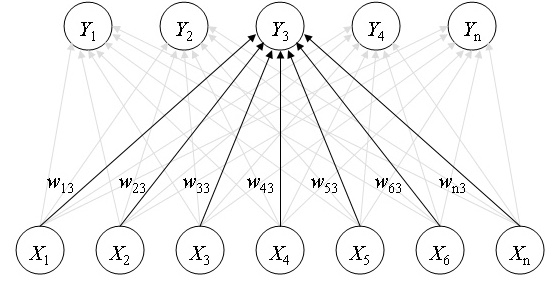
\includegraphics[scale=0.4]{1.jpeg}
\caption{Self-Organizing Map Architecture}
\label{SOM}
\end{figure}
\subsection{Multilayer Perceptron}
This section only if we decide to do this finally.

\section{Experimentation}

\subsection{Dataset}
\subsection{Data Labelling}
We might need to hand label the attributes as a base line to check the accuracy of out system.
\subsection{Results}
Clustering accuracy table, scatter plots etc.

\section{Limitations}
No many to one mapping and anything else you can think of.

\section{Future Work}
% if have a single appendix:
%\appendix[Proof of the Zonklar Equations]
% or
%\appendix  % for no appendix heading
% do not use \section anymore after \appendix, only \section*
% is possibly needed

% use appendices with more than one appendix
% then use \section to start each appendix
% you must declare a \section before using any
% \subsection or using \label (\appendices by itself
% starts a section numbered zero.)
%



%\appendices
%\section{Proof of the First Zonklar Equation}
%\blindtext

% use section* for acknowledgement
%\section*{Acknowledgment}


%The authors would like to thank...


% Can use something like this to put references on a page
% by themselves when using endfloat and the captionsoff option.
%\ifCLASSOPTIONcaptionsoff
%  \newpage
%\fi



% trigger a \newpage just before the given reference
% number - used to balance the columns on the last page
% adjust value as needed - may need to be readjusted if
% the document is modified later
%\IEEEtriggeratref{8}
% The "triggered" command can be changed if desired:
%\IEEEtriggercmd{\enlargethispage{-5in}}

% references section

% can use a bibliography generated by BibTeX as a .bbl file
% BibTeX documentation can be easily obtained at:
% http://www.ctan.org/tex-archive/biblio/bibtex/contrib/doc/
% The IEEEtran BibTeX style support page is at:
% http://www.michaelshell.org/tex/ieeetran/bibtex/
%\bibliographystyle{IEEEtran}
% argument is your BibTeX string definitions and bibliography database(s)
%\bibliography{IEEEabrv,../bib/paper}
%
% <OR> manually copy in the resultant .bbl file
% set second argument of \begin to the number of references
% (used to reserve space for the reference number labels box)
\begin{thebibliography}{1}

\bibitem{IEEEhowto:kopka}
H.~Kopka and P.~W. Daly, \emph{A Guide to \LaTeX}, 3rd~ed.\hskip 1em plus
  0.5em minus 0.4em\relax Harlow, England: Addison-Wesley, 1999.

\end{thebibliography}

% biography section
% 
% If you have an EPS/PDF photo (graphicx package needed) extra braces are
% needed around the contents of the optional argument to biography to prevent
% the LaTeX parser from getting confused when it sees the complicated
% \includegraphics command within an optional argument. (You could create
% your own custom macro containing the \includegraphics command to make things
% simpler here.)
%\begin{biography}[{\includegraphics[width=1in,height=1.25in,clip,keepaspectratio]{mshell}}]{Michael Shell}
% or if you just want to reserve a space for a photo:

\begin{IEEEbiography}[{\includegraphics[width=1in,height=1.25in,clip,keepaspectratio]{picture}}]{John Doe}
\blindtext
\end{IEEEbiography}

% You can push biographies down or up by placing
% a \vfill before or after them. The appropriate
% use of \vfill depends on what kind of text is
% on the last page and whether or not the columns
% are being equalized.

%\vfill

% Can be used to pull up biographies so that the bottom of the last one
% is flush with the other column.
%\enlargethispage{-5in}




% that's all folks
\end{document}


